\documentclass[article,9pt,twocolumn,twoside]{rilabRxiv}
% Use the documentclass option 'lineno' to view line numbers
\setlength{\marginparwidth}{2cm}
\usepackage[textsize=tiny,colorinlistoftodos]{todonotes} % comments in margins
\definecolor{cornflowerblue}{rgb}{0.39, 0.58, 0.93}
\usepackage{blindtext}

\usepackage{hyperref}
%interwordspace: \the\fontdimen2\font \\

%interwordstretch: \the\fontdimen3\font \\

%emergencystretch: \the\emergencystretch\par
%\blindtext

%%%%%%%Add comments in color
\newcommand{\ms}[1]{{\small \textcolor{green}{#1}}}
\newcommand{\jri}[1]{{\small \textcolor{red}{#1}}}
\newcommand{\citex}[1]{{\small \textcolor{red}{CITE(#1)}}}
\newcommand{\X}{{\textcolor{red}{X}}}

\newcolumntype{b}{X}
\newcolumntype{s}{>{\hsize=.5\hsize}X}

% Set supplement numbers to S and start counting newly
\newcommand{\beginsupplement}{%
        \setcounter{table}{0}
        \renewcommand{\thetable}{S\arabic{table}}%
        \setcounter{figure}{0}
        \renewcommand{\thefigure}{S\arabic{figure}}%
     }


\title{Method of Analysis of Multi-parent Mapping Populations Affects Detection of QTL}

\author[$\ast$,1]{Odell, S. G.}
\author[$\dagger$]{Praud, S.}
\author[$\ast$,$\ddagger$]{Ross-Ibarra, J.}
\author[$\ast$,$\ddagger$]{Runcie, D.}


\affil[$\ast$]{Dept. of Plant Sciences and Center for Population Biology, University of California, Davis, CA, USA}
\affil[$\dagger$]{Limagrain, Chappes, France}
\affil[$\ddagger$]{Genome Center, University of California, Davis, CA, USA}


\keywords{QTL, MAGIC}

\runningtitle{Running title} % For use in the footer

%% For the footnote.
%% Give the last name of the first author if only one author;
% \runningauthor{Odell}
%% last names of both authors if there are two authors;
% \runningauthor{FirstAuthorLastname and SecondAuthorLastname}
%% last name of the first author followed by et al, if more than two authors.
\runningauthor{Odell \textit{et al.}}

%%% Abstract %%%%%%%%%%%%%%%%%%
\begin{abstract}
The search for quantitative trait loci (QTL) that explain complex traits such as yield and drought tolerance has been ongoing in all crops. Methods such as bi-parental QTL mapping and genome-wide association studies (GWAS) each have their own advantages and limitations. Multi-parent advanced generation inter-crossing (MAGIC) contain more recombination events and genetic diversity than bi-parental mapping populations and reduce the confounding effect of population structure that is an issue in association mapping populations. Here we discuss the results of using a MAGIC population of doubled haploid (DH) maize lines created from 16 diverse founders to perform QTL mapping, comparing QTL identified using a 600K SNP array to those found using founder probabilities and haplotype probabilities generated by determining the regions of the MAGIC DH lines that were derived from the 16 founders and by identifying regions of identity-by-descent (IBD) between the 16 founders, respectively. The three methods have differing power and resolution for detecting QTL for a variety of agronomic traits. This highlights the importance of considering different approaches to analyzing genotypic datasets, and shows the limitations of binary SNP data for identifying multi-allelic QTL.
\end{abstract}
%%%%%%%%%%%%%%%%%%%%%%%%%%


\setboolean{displaycopyright}{true}

\begin{document}

\maketitle
\thispagestyle{firststyle}
%\firstpagefootnote
\correspondingauthoraffiliation{
Dept. of Plant Sciences, University of California, Davis, CA, USA
E-mail: sgodell@ucdavis.edu}
\vspace{-11pt}%

\section{Introduction}
%\subsection{First part}
The study of evolutionary quantitative genetics requires the ability to link differences in phenotype to genotypic variation. Natural and artificial selection acts on phenotypes, but only heritable phenotypic variation will result in changes in population means. Maize presents an excellent model organism to answer these questions due to the combination of extensive genetic and phenotypic resources, and the ability to create mapping populations. In addition, maize is one of the most widely produced crops in the world and is a major source of calories for millions of people. Decades of research into maize genetics have resulted in the identification of many quantitative trait loci (QTL) that explain variation in phenotypes such as yield, flowering time, and plant height (\citep{RN40};\citep{RN42};\citep{RN85}). Such traits are extremely agronomically important. They are also crucial plant phenotypes in terms of fitness and local adaptation.
Researchers have been able to discover large-effect QTL for a number of agronomic traits through the use of different types of mapping populations \citep{RN93}. The choice of any population comes with associated advantages and limitations. In particular, they tend to vary in two main characteristics: (1) their ability to capture genetic diversity and (2) their power to detect QTL of small effect. Multi-parent Advanced Generation Intercross (MAGIC) populations have been used in breeding to increase the genetic diversity and number of recombination events included in a mapping population compared to biparental populations \citep{RN8}[give more example citations]. Compared to genome-wide association panels, MAGIC populations have more power to detect rare alleles (i.e. alleles that are only present in one of the parents) and can better estimate allelic effects because the crossing scheme increases the frequency of all parental alleles to be approximately equal. Simulations of an 8-parent MAGIC population showed that sample sizes of 300 could detect QTL accounting for 12\% of variance with a power of 82\% \citep{RN65}. Lastly, a MAGIC population avoids confounding due to population structure that is encountered with GWAS because the pedigree of the lines is known.
In this study, we utilized a MAGIC population of about 400 doubled-haploid lines derived from 16 inbred maize parents developed by Limagrain to understand how methods of representing genotypic data can impact the identification of QTL. Extensive genetic resources already exist for maize, but do not possess the same diversity and statistical power as the Biogemma MAGIC population. A maize nested association mapping (NAM) population exists, consisting of RIL populations derived from 25 inbred parents crossed to B73 \citep{RN75}.  Only two inbred parents overlap between the NAM and Biogemma MAGIC populations (B73 and Oh43), and compared to the NAM, the MAGIC population can have similar power to the NAM using half the number of samples \citep{RN65}. Likewise, another maize MAGIC population has previously been created, which overlaps by three parents (A632, B73, and B96) \citep{RN65}. However, the previous MAGIC is derived from 8 inbred maize parents instead of 16, and consists of RILs, not doubled haploids, so some residual heterozygosity may exist.  For these reasons, the Biogemma MAGIC population has great potential to reveal new insights into the genetic control of quantitative traits in maize. It also serves a reliable standard for QTL mapping method comparision because DH lines were used and the crossing scheme ensured that there is a reasonably even distribution of the 16 founders within the population (supplemental figure?)

\lettrine[lines=2]{\color{color2}A}{} good introduction is very important.
%This is how you can \citet{hufford2012comparative} in line or as reference in
% the end \citep{bourne2017ten}.
%\subsection{Second part}
%\blindtext
\section{Materials and Methods}
\label{sec:materials:methods}
\subsection{Genotype Data}
The MAGIC population was derived from 16 inbred maize parents representing the
 diversity of European flint and U.S. dent heterotic groups. The 16 founder
  lines were crossed in a funnel crossing scheme, and then the resulting
   synthetic population was intercrossed for 3 generations with around 2000
    individuals per cycle (Figure \ref{fig:figure1}A). Finally, 800 lines were selected from the synthetic
     population to create doubled haploids (DH), resulting in 550 MAGIC DH
      lines at the end of the process. The 16 founder lines and the MAGIC DH
       lines were all genotyped with the Affymetrix 600K Axiom SNP array. In
       addition, the 16 founder lines were sequenced with Illumina short-read
       sequencing to a depth of [?]x, resulting in 45.4 millions SNPs and
       5.4 indels after filtering using GATK best practices.


\subsection{Phenotype Data}
The MAGIC DH lines were crossed to a tester MBS84 to produce 344 hybrids.
 Due to variation in flowering time, a subset of the lines could not be crossed
  to the tester. The hybrids were grown in the field in Blois, France in 2014.
   For each genotype, two blocks of around 80 plants were grown under
   well-watered conditions. Measured phenotypes included days to anthesis (DTA),
    days to silking (DTS), plant height, percent harvest grain moisture, grain
     yield, and thousand kernel weight (adjusted to 15\% humidity), where values
      were averaged over blocks. Both flowering time phenotypes were measured as
       the sum of degree days since sowing with a base temperature of
        6$^{\circ}$C (48$^{\circ}$F). Days to anthesis was considered as the
         growing degree days until 50\% of plants in a block were flowering at
          25\% of the central tassel spike.

\subsection{Calculation and Validation of Founder Probabilities}
The package R/qtl2 \citep{RN39} was used to determine founder probabilities of the DH
 lines using the 600K genotype data and the cross type ``riself16''. Due to the
  fact that the actual crossing scheme and the cross type input into R/qtl2
   differed, we wanted to assess the accuracy of the founder probabilities.
    This was done by simulating lines using the actual crossing scheme and
     assessing the performance of the calc\_genoprobs function of R/qtl2 in
      correctly identifying the founder genotype (Figure \ref{fig:figure1}). We developed an R package,
       magicsim (\url{https://github.com/sarahodell/magicsim}), to simulate the lines using the maize genetic map
        from Ogut et al. 2015 to generate approximate recombination rates across
         the chromosome. For 400 simulated lines, 99.6\% of SNPs were correctly
          assigned to the founder genotype.

\begin{figure*}[ht!]
\centering
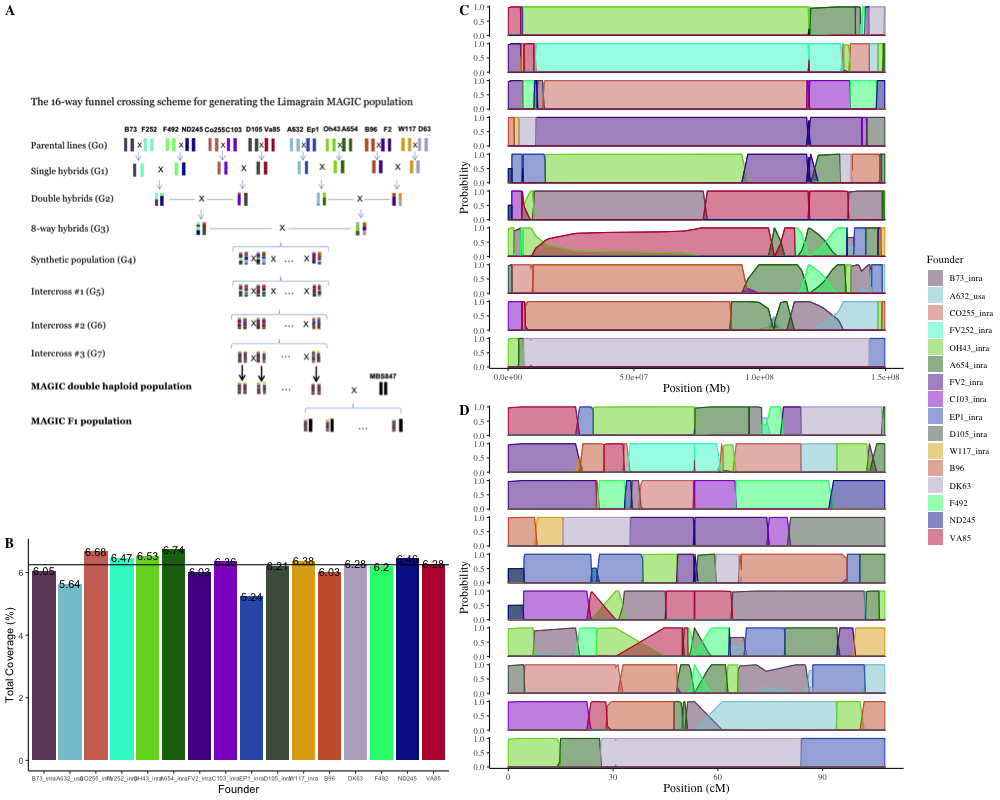
\includegraphics[width=\textwidth,height=14cm]{figures/Methods_Fig1.png}
\caption{\textbf{Structure, diversity, and founder representation of the MAGIC population}(\textbf{A}) The crossing scheme of the MAGIC population. (\textbf{B}) Founder probabilities for 10 MAGIC DH lines on chromosome 10 in physical distance. (\textbf{C}) The number of unique haplotype groups among the 16 founder lines across chromosome 10. (\textbf{D}) Founder probabilities for 10 MAGIC DH lines on chromosome 10 in genetic distance.}
\label{fig:figure1}
\end{figure*}

\subsection{Calculation of Haplotype Probabilities}
The use of founder probabilities makes the assumption that all 16 founders have
distinct haplotypes. This assumption is not realistic, especially considering the
known varying degrees of relatedness between the founders. The identification of
regions of shared genetic sequence between founder pairs would allow for the collapsing
of founder probabilities into haplotype probabilities. These haplotype probabilities
have the potential to increase statistical power by reducing the number of tests
performed in QTL mapping. Areas of uncertainty in founder probabilities of the
DH lines were associated with regions of identity-by-descent (IBD) between two or
 more founder lines in that region of the chromosome. Identity-by-state (IBS) was measured from the
600K genotype data of the founders using the software GERMLINE with the paramaters
```-wextend```,```--min\_m 1``, and ```--err\_hom 4``` as a proxy for IBD. In order
 to assess the quality of predicted IBD regions, we also identified IBD regions
 using the founder WGS data. This was done using two separate softwares. GERMLINE
 was run using the same parameters as above on the WGS data with all sites with
 missing data removed, resulting in a total of 16.9 million SNPs for comparison
 of sequence similarity. The software IBDSeq was run in addition using the full
 45.4 million sites in the WGS data. Comparision of overlap between pairwise IBD
 regions among the three methods showed [... significant overlap between the 600K
 and WGS data... actual numbers]. Haplotype blocks were created by grouping regions
  of pairwise IBD across the 16 founders. Within blocks, the founder probabilities
  for founders that were in  IBD were summed to obtain haplotype probabilities.
  This resulted in haplotype blocks with the number of unique haplotypes within
   blocks ranging from [2?] to 16.

\subsection{Association and QTL Mapping}
The R package GridLMM [] was used to run association mapping using the three
 different methods of representing the genotype data. The function GridLMM\_ML was
 used with the "ML" option. The model for each was
\begin{equation}
\label{eqn:gridlmm}
 Y = X\beta + Zu + \epsilon
\end{equation}

where $Y$ is the response variable, $X$ is the genotype matrix, $\beta$,
is the effect size, $Z$ is the design matrix, $u$ is the random
effects, and $\epsilon$ is the error. Significance cutoffs for p-values were
 obtained using permutation testing, taking the 5\% cutoff from 1000 randomized
  permutations for each method. Code for the analyses can be found [github link].

\subsection{Method Comparison}
The results of the three methods of identifying QTL were compared using two main
criteria: (i) presence or absence of identified QTL peaks and (ii) the resolution
of those QTL peaks. The GWAS methods should be most powerful at identifying QTL
for which the causal variant is biallelic and the tagged SNP is in tight LD with
the causal varaint. However, for multi-allelic QTL or QTL for which LD is low
between tagged SNPs, this method begins to lose power. Founder probabilities increase
the odds of detecting both QTL that are multi-allelic and QTL whose causal variant
is not in tight LD with any one tagged SNP [Supplemental Figure?]. Lastly,
haplotype probabilities potentially improve on the power of founder probabilities
to detect QTL that meet the above criteria by reducing the number of test. However,
haplotype probabilities also may obscure the signal of some QTL if founders are
called as being in IBD with one another when they actually differ for the causal
variant. Due to the fact that the founder and haplotype probabilities
take into account recent recombination events, whereas the GWAS method only uses
historical recombination, we predicted that founder and haplotype mapping would
result in higher resolution around QTL peaks. Higher resolution QTL are ideal in
that it makes it easier to narrow down candidate genes and potential causal variants
when the significant window is smaller.

%\textbf{General}
%\begin{table}[htbp]
%\centering
%\caption{\bf Parameters and variables}
%\begin{tableminipage}{0.5\textwidth}
%\begin{tabularx}{\textwidth}{sb}
%\hline
% Variable & Description \\
%\hline
%$N_{anc}$ & Population size at equilibrium \\
%$N_{final}$ & Population size after 0.1 * $N_{anc}$ generations \\
%$N_{bottlenck}$ & Population size during bottleneck \\
%$\psi$ & Genetic background proportion \\
%$\sigma_m$ & Standard deviation of effect sizes of new mutations \\
%$V_S$ & Strength of stabilizing selection \\
%$V_{G0}$ & Genetic variance at equilibrium\\
%\hline
%\end{tabularx}
%  \label{tab:shape-functions}
%\end{tableminipage}
%\end{table}

%\subsection{Experiment 1}
%\blindtext

%\subsubsection{Experiment 2}
%This is an example equation

%\begin{equation}
%\label{eqn:fitness}
%w =exp [-\frac{(z-z_{opt})^2}{2V_S}]
%\end{equation}

%\blindtext
%%%%%%%%%%%%%%%%%%%%%%%%%%%%%%%%%%%%%%%%%%%%%%%%%%%%%%
\section{Results}
%%%%%%%%%%%%%%%%%%%%%%%%%%%%%%%%%%%%%%%%%%%%%%%%%%%%%%

\subsection{MAGIC Population}
Analysis of the MAGIC population showed that the representation of the 16 founders in the MAGIC DH lines was relatively even, with the highest percentage founder, A654, representing 6.741\% and the lowest percentage founder, EP1, representing 5.237\% (Supplemental Figure). Across all regions of the each chromosomes, for 99\%(?) of markers in the 600K array, at least one DH line was derived from each of the 16 founders with high confidence (greater than 0.9 probability) (Supplemental Figure). One notable exception was on chromosome 6, where a region [location] had no representation from [founders]. This may be due to these founders being in close IBD with another founder, resulting in uncertainty in the founder probablities. Another possible explanation is that there was selection against theese founders during the breeding process. This region approximately corresponds to the NOR region [citation].


The founder probabilities determined using R/qtl2 were able to assign founders to the DH lines with high confidence (>0.90) for [percentage] of the 10 chromosomes of maize.

\subsection{Simulation and Validation of Founder Probabilities}
Using the package we created, magicsim, we simulated chromosome 10 for 1000 MAGIC DH lines following the crossing scheme used for the actual population. We then the ran R/qtl2 on these simulated lines to obtain founder probabilities and compared these probabilities to the known founder identities of the simulated lines. In total, for sites for which R/qtl2 was able to assign founder probabilities, the maximum probability founder matched the actual founder for 99.8\% of sites. This reinforced our confidence in the founder probabilties obtained from the actual data.

\subsection{Phenotype Data}
The distribution of the six measured phenotypes were approximately normal (Figure \ref{fig:figure2}).

\begin{figure}[ht]
\centering
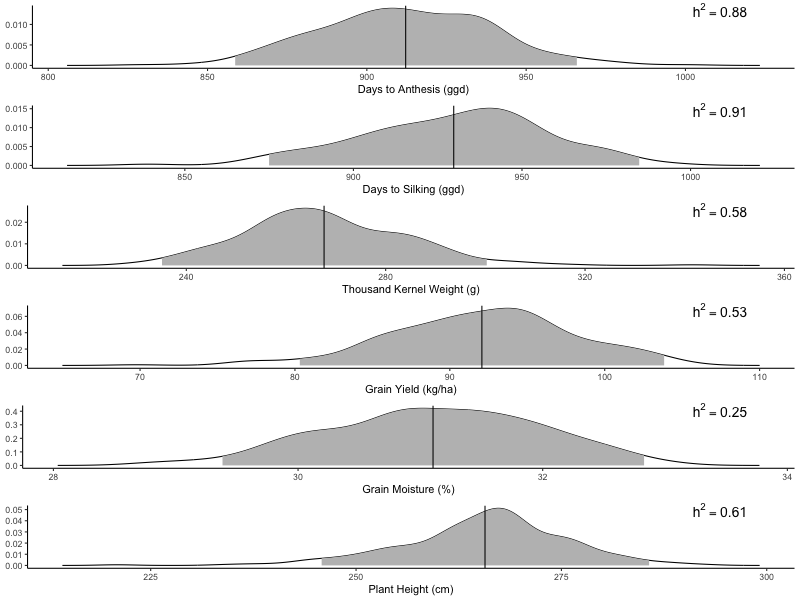
\includegraphics[width=\linewidth]{figures/Methods_Fig2.png}
\caption{\textbf{Distribution of phenotypes} The density plots of the six measured phenotypes. The vertical bar represents the mean, and the grey shading shows two standard deviations. The heritability of each trait is shown on the right.}
\label{fig:figure2}
\end{figure}

\subsection{QTL Mapping and Association Mapping}
The three methods varied both in their ability to identify QTL and the resolution of those QTL.
\subsection{Variation around \emph{vgt1}}
A previously characterized QTL, \emph{vgt1} is associated with variation in flowering time [citations]. An earlier flowering phenotype is strongly correlated with a MITE insertion about 70kb upstream of the flowering time regulator, \emph{ZmRAP2.7}, an \emph{APETALA}-like transcription factor [].

\begin{figure*}[hb!]
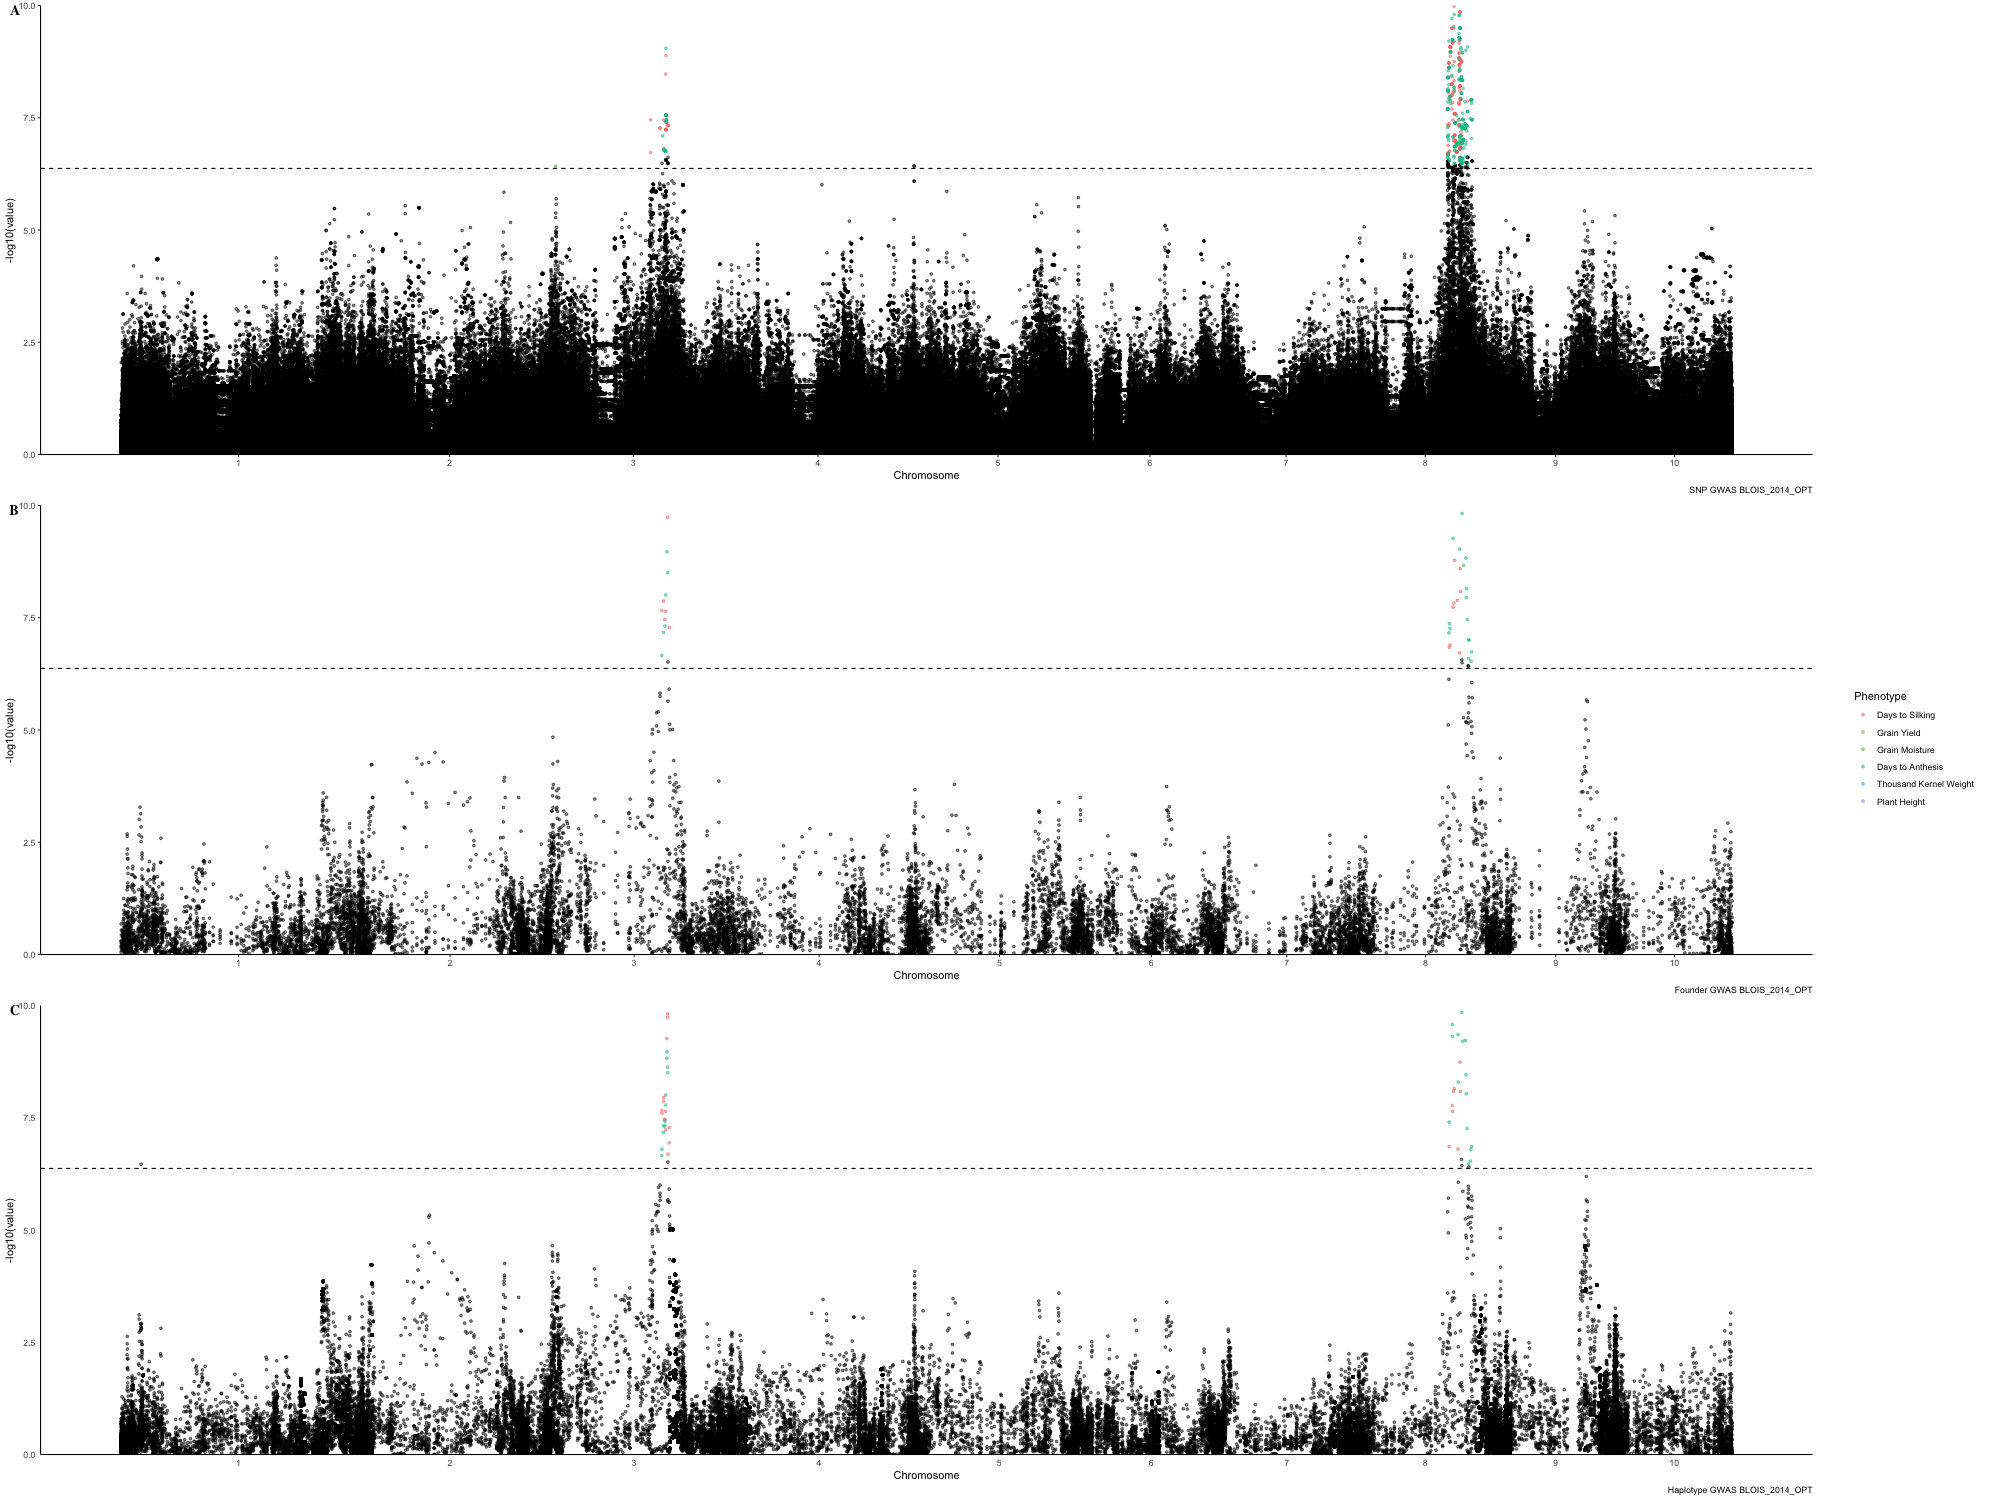
\includegraphics[width=\textwidth,height=14cm]{figures/Methods_Fig3.png}
\caption{\textbf{Results of three methods of QTL identification} Colored points represent signficant SNPs above the 5\% signficance threshold from 1000 random permutations \textbf{top} GWAS results using the 600K SNP array. \textbf{middle} Results from QTL mapping using founder probabilities \textbf{bottom} Results from QTL mapping using haplotype probabilities}
\label{fig:figure3}
\end{figure*}

%\blindtext

%\blindtext
%\blindtext
%\blindtext
%\blindtext
%%%%%%%%%%%%%%%%%%%%%%%%%%%%%%%%%%%%%%%%%%%%%%%%%%%%%%
\section{Discussion}
%%%%%%%%%%%%%%%%%%%%%%%%%%%%%%%%%%%%%%%%%%%%%%%%%%%%%%
\subsection{Some more test}
\blindtext
\blindtext


\subsection{another figure}
This is a full size figure (Figure \ref{fig:S1}) just add stars to the figure


\section{Acknowledgments}
We acknowledge the support of our coffee maker that made this work possible

\bibliography{magic_tex}

%\pagebreak
\onecolumn
\section*{Supplement}



\beginsupplement


\blindtext
\begin{figure*}[h!]
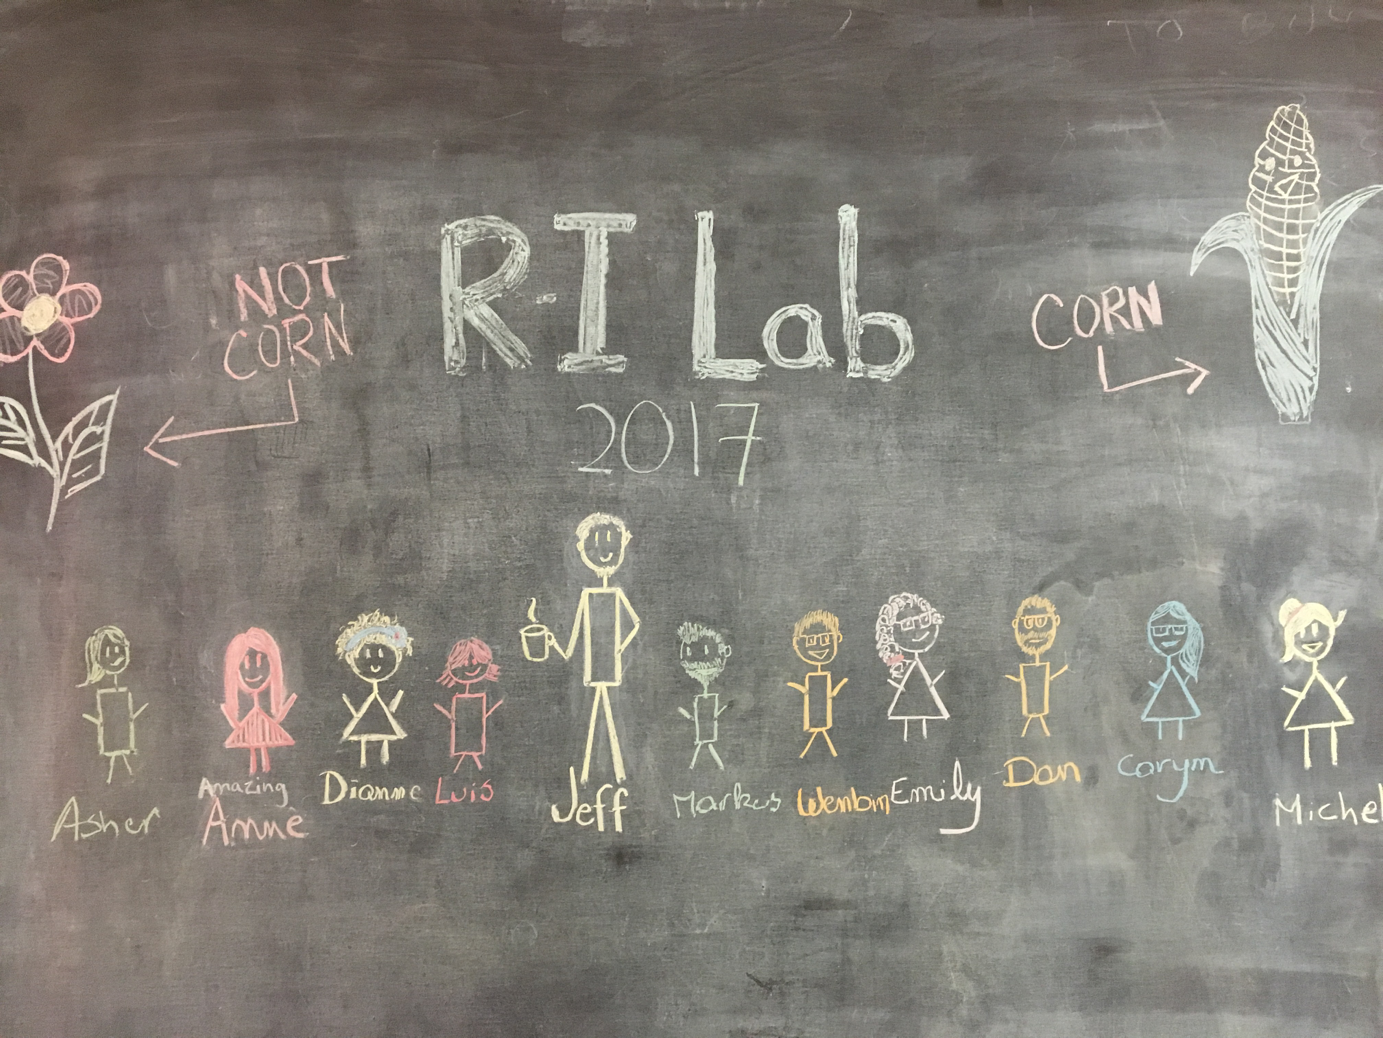
\includegraphics[width=.9\linewidth]{figures/lab_group.png}
\caption{\textbf{Supplemental figure} Test test test}
\label{fig:S1}
\end{figure*}
\pagebreak




\begin{table*}[htbp]
\centering

\caption{\bf Shrink a large table to fit the page}
%\begin{adjustbox}{totalheight=\textheight-2\baselineskip}
\begin{tableminipage}{\textwidth}
\begin{small}
\begin{tabularx}{\textwidth}{sb}
\hline
Parameter & Description \\
\hline
\textbf{Adaptation} & \textbf{Trait related parameters} \\
\hline
Time to optimum & Generations until new optimum is reached \\
Adaptation rate (haldane) & Adaptation rate until new optimum is reached. Calculated as $rate(h) = \frac{\frac{ln(x_2)}{sd_{x_{12}}}-\frac{ln(x_1)}{sd_{x_{12}}}}{t_2-t_1}$ \\
Final genetic variance & Genetic variance in the final generation \\
\textbf{Fixations} & \textbf{Mutations that fix after the optimum shift} \\
\hline
From new mutations (\#) & Sum of fixed mutations in the final population that were already segregating before  the optimum shift \\
From standing variation (\#) & Sum of fixed mutations in the final population that arose after the optimum shift \\
Max. effect size & Maximal effect size of all fixations \\
Mean effect size & Mean effect size of all fixations \\
Mean effect size of negative fixations & Mean effect size of negative mutations \\
Mean effect size of positive fixations & Mean effect size of positive mutations \\
Mean emergence time & Mean generation when a mutation arose that fixed in the last 0.1 N generations \\
Mean fixation time & Mean generation in which a mutation fixed \\
Min. effect size & Minimal effect size of all fixations \\
Negative (\#) & Sum of fixed mutations with negative effects in the final population \\
New/standing fixations & Ratio of mutations from new mutations vs. standing mutations  \\
Proportion negative & Proportion of negative fixations from all mutations \\
Positive (\#) & Sum of fixed mutations with positive effects in the final population \\
SD of effect sizes & Standard deviation of effect sizes of all fixations \\
SD of negative effect sizes & Standard deviation of effect sizes of negative fixations \\
SD of positive effect sizes & Standard deviation of effect sizes of positive fixations \\
Total (\#) & Sum of fixed mutations in the final population \\
\textbf{Sweeps} & \textbf{Mutations that fix faster than 99\% of neutral fixations} \\
\hline
Hard sweeps (\#) & Sum of selective sweeps from new mutations \\
Proportion of hard sweeps & Porportion of hard selective sweeps of all selective sweeps \\
Proportion of sweeps from standing & Proportion of selective sweeps from stainding variation of all selection sweeps \\
Sweeps (\#) & Sum of selective sweeps \\
Sweeps from standing variation (\#) & Sum of selective sweeps from mutations that were already segregating before  the optimum shift \\
Sweeps/fixations & Ratio of sweeps vs. fixations \\
\textbf{Segregating sites} & \textbf{Mutations that segregate in the final generation} \\
\hline
Max. effect size & Maximal effect size of segregating sites \\
Mean effect size & Mean effect size of segregating sites \\
Mean effect size of negative sites & Mean effect size of segregating sites with negative effects \\
Mean effect size of positive sites & Mean effect size of segregating sites with positive effects \\
Mean frequency of all sites & Mean allele frequency of segregating sites \\
Mean frequency of negative sites & Mean allele frequency of segregating sites with negative effects \\
Mean frequency of positive sites & Mean allele frequency of segregating sites with positive effects \\
Min. effect size & Minimal effect size of segregating sites \\
Negative (\#) & Sum of segregating sites with negative effect \\
Positive (\#) & Sum of segregating sites with positive effect \\
Proportion of negative sites & Proportion of segregating sites with negative effect of all segregating sites \\
Standard deviation of effect sizes & Standard deviation of effect sizes of all segregating sites \\
Total (\#) & Sum segregating sites in the final generation \\
\hline

\end{tabularx}
  \label{tab:parameter_list}
  \end{small}
\end{tableminipage}

%\end{adjustbox}
\end{table*}


\end{document}
